\documentclass[11pt, oneside]{article} 
\usepackage{geometry}
\geometry{letterpaper} 
\usepackage{graphicx}
	
\usepackage{amssymb}
\usepackage{amsmath}
\usepackage{parskip}
\usepackage{color}
\usepackage{hyperref}

\graphicspath{{/Users/telliott/Github/number_theory/png/}}
% \begin{center} \includegraphics [scale=0.4] {gauss3.png} \end{center}

\title{Chinese remainder theorem}
\date{}

\begin{document}
\maketitle
\Large

The Chinese remainder theorem is sometimes abbreviated as the CRT.

\begin{quote}There are certain things whose number is unknown. Repeatedly divided by 3, the remainder is 2; by 5 the remainder is 3; and by 7 the remainder is 2. What will be the number?  -- Sun Tsu Suan-Ching\end{quote}

\url{https://www.cut-the-knot.org/blue/chinese.shtml}

Consider $n$ and its prime factors (or even combinations of prime factors, as long as each value is coprime), then

\begin{quote}the tuple of remainders from the modulus operation on $n$ with its coprime factors is unique\end{quote}

Not only is the tuple unique, but 

\begin{quote}it can be used to reconstruct the result of the modulus operation on $n$\end{quote}
    
Therefore, that operation can be replaced by easier operations on each of the smaller factors.  This result is used to simplify some operations with RSA keys, as we'll see.

\subsection*{examples}
Let $n = 20$ and consider the coprime factors $4$ and $5$:

\begin{verbatim}
1 2 3 4 5 6 7 8 9 0 1 2 3 4 5 6 7 8 9 0
      |       |       |       |       | 
1 2 3 0 1 2 3 0 1 2 3 0 1 2 3 0 1 2 3 0   mod 4
        |         |         |         |
1 2 3 4 0 1 2 3 4 0 1 2 3 4 0 1 2 3 4 0   mod 5
\end{verbatim}
  
For each number in the range $[1..n]$ write the result mod $4$ or $5$ as a tuple:

\begin{verbatim}
(1,1),(2,2),(3,3),(0,4),(1,0)
(2,1),(3,2),(0,3),(1,4),(2,0)
(3,1),(0,2),(1,3),(2,4),(3,0)
(0,1),(1,2),(2,3),(3,4),(0,0)
\end{verbatim}

Each one is unique.

\begin{center} 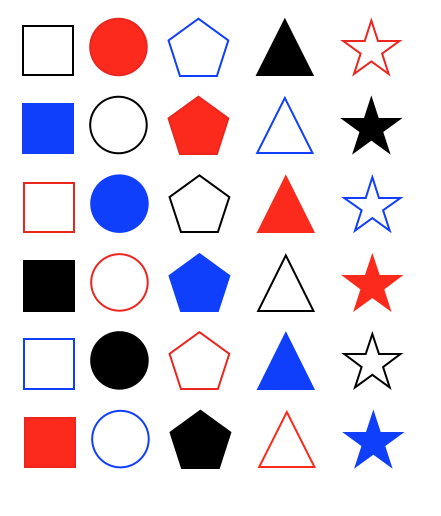
\includegraphics [scale=0.4] {shapes.png} \end{center}

In the picture above, we have 

$\circ$ \ 5 distinct shapes

$\circ$ \ 3 different colors

$\circ$ \ 2 states, either filled or empty

As you can see, there are precisely $30$ possible types.  

For example, each shape can be one of three colors, filled or empty, so there are 6 possibilities for each of the five shapes.  This is simply a consequence of the fact that

\[ 5 \cdot 3 \cdot 2 = 30 \]

Since there are 30 numbers in $[1..30]$, there is exactly one type for each number.

\subsection*{theorem}

If $N$ is composed of coprime factors

\[ N = p \cdot q \cdot r \dots \]

and $n$ is in the range $[1..N]$.

Suppose $n$ has the set of remainders with those factors:

$\circ$ \ $n = a$ mod $p$

$\circ$ \ $n = b$ mod $q$

$\circ$ \ $n = c$ mod $r$

Then this tuple $(a,b,c)$ uniquely identifies $n$.

\subsection*{example}

Suppose $N = 60$, so 

\[ 30 = 2 \cdot 3 \cdot 5 \]

Make a table of remainders:


\begin{verbatim}
    1  2  3  4  5  6  7  8  9 10 11 12 13 14 15
2:  1  0  1  0  1  0  1  0  1  0  1  0  1  0  1
3:  1  2  0  1  2  0  1  2  0  1  2  0  1  2  0
5:  1  2  3  4  0  1  2  3  4  0  1  2  3  4  0

   16 17 18 19 20 21 22 23 24 25 26 27 28 29 30
2:  0  1  0  1  0  1  0  1  0  1  0  1  0  1  0
3:  1  2  0  1  2  0  1  2  0  1  2  0  1  2  0
5:  1  2  3  4  0  1  2  3  4  0  1  2  3  4  0
\end{verbatim}

Any particular triplet of remainders is unique, say:  $(1,1,3) \rightarrow 13$.

This is also true if the factors are not prime but simply co-prime:

\begin{verbatim}
    1  2  3  4  5  6  7  8  9 10 11 12 13 14 15
5:  1  2  3  4  0  1  2  3  4  0  1  2  3  4  0
6:  1  2  3  4  5  0  1  2  3  4  5  0  1  2  3

   16 17 18 19 20 21 22 23 24 25 26 27 28 29 30
5:  1  2  3  4  0  1  2  3  4  0  1  2  3  4  0
6:  4  5  0  1  2  3  4  5  0  1  2  3  4  5  0
\end{verbatim}

\subsection*{solving the system}

I picked a column at random from above.  

Consider the following table of remainders (congruences):
\[ x \equiv 1 \ \text{(mod 2)} \]
\[ x \equiv 1 \ \text{(mod 3)} \]
\[ x \equiv 3 \ \text{(mod 5)} \]

The CRT says that this tuple uniquely determines $x$.  We can actually solve the system for $x$.

It's kind of spammy, but I found out how to do this here

\url{https://brilliant.org/wiki/chinese-remainder-theorem}

Start with the largest modulus $x \equiv 3 \ \text{(mod 5)}$.  Re-write this as: 
\[  x = 5j + 3 \]

For some integer $j$.   Substitute into $x \equiv 1 \ \text{(mod 3)}$:
\[  5j + 3 = 1 \ \text{(mod 3)}  \]

Solve for $j$:
\[  5j = 1 \ \text{(mod 3)}  \]
\[  2j = 1 \ \text{(mod 3)}  \]
\[  j = 2 \ \text{(mod 3)}  \]
A multiplication table can help with the last step above.

Rewrite this as a congruence relation for some integer $k$.
\[   j = 3k + 2 \]

Back-substitute:
\[  x = 5j + 3 \]
\[  x = 5(3k + 2) \]
\[  x = 15k + 13 \]
Now we have $x$ in terms of $k$.  We are done with equation 2.

Repeat the cycle by substituting into $x \equiv 1 \ \text{(mod 2)}$ and solve for $k$.
\[  15k + 13 = 1 \ \text{(mod 5)}  \]
\[  k + 3 = 1 \ \text{(mod 5)} \]
\[  k = -2 = 0 \ \text{(mod 2)} \]

which means that
\[  k = 2m \]

for some m.  And then
\[  x = 15k + 13 \]
\[  x = 15(2m) + 13 \]
\[  x = 13 \ \text{(mod 30)}  \]

\subsection*{riddle}

The answer is 

\begin{verbatim}
>>> for i in range(106):
...     t = (i,i%3,i%5,i%7)
...     print(t)
...     if t[1:] == (2,3,2):
...         break
... 
..
(23, 2, 3, 2)
\end{verbatim}


\end{document}